\documentclass{tufte-handout}
\usepackage{graphicx}
\usepackage{exercise}
\usepackage{enumerate}
\usepackage{amsmath,amssymb,amsthm}
\usepackage{enumitem}
\newcommand{\bi}{\begin{itemize}}
\newcommand{\ei}{\end{itemize}}
\newcommand{\be}{\begin{enumerate}}
\newcommand{\ee}{\end{enumerate}}
\newcommand{\beq}{\begin{equation}}
\newcommand{\eeq}{\end{equation}}

\title{Module 1 Exercises: Interactions}
\begin{document}

\maketitle

\vspace{0.1in}


%%%%%%%%%%%%%%%%%%%%%%
% SECTION 1: VECTOR OPERATIONS
%%%%%%%%%%%%%%%%%%%%%%

\section{How to do Interactions 1}

This set of exercises is long.  If you {\it really} know your stuff you can probably easily complete it in 9 hours, but if you're learning new stuff in here there is no way you'll be able to get every problem done in 9 hours.

So you have two choices.  The {\it bad} choice would be to bang your head against this assignment until you have done every problem.  We will not stop you from doing this.  But we will discourage you.

The {\it good} choice would be to spend a good solid 9 hours on it (including the time you're watching videos), but do so in a way that maximizes your learning of the full range of material that's represented here.  That might look something like this:

\begin{enumerate}
\item Start on this assignment today.  9 hours spread over Thursday, Friday, Saturday, and Sunday is not unreasonable.  9 hours on one day is insane and highly unproductive.
\item Watch the videos on vectors (at 2x speed or 0.5x speed, as suits your needs).
\item Talk to a ninja or an instructor if you are confused.
\item Do a few of the vector problems to make sure you at least have a general handle on it.  Choose questions that challenge you, and that cover different aspects of the section.
\item Talk to a ninja or instructor if you are confused.
\item Watch the videos on force models (again, at a speed and skipping level that suits you)
\item Talk to a ninja or instructor if you are confused.
\item Do a few of the force model questions; again, choose questions that challenge you, and that cover different aspects of the section.
\item You know what comes next here.
\item Continue in this mode for the remainder of the assignment.
\item Once you've done a few problems from each section, go back and start over again, doing additional problems.
\item Repeat until you (1) feel like you totally have stuff under control, or (2) have spent a solid 9 hours on the assignment.  \item If you get to 9 hours of good, solid, work, and you've sought help when you felt lost, and you still feel lost after we do in-class activities on Monday, then {\bf please talk to us about it.}
\item {\it Please do not bang your head on a question.  If you are lost on a question, ask for help!}
\end{enumerate}


\section{Vectors and Vector Operations: Cartesian}

You've probably dealt with vectors some before. Vectors can be thought of both in the physical world (e.g., position vectors), as well as in more abstract spaces, as we'll discuss in future modules. They are a pretty critical building block throughout engineering, math, and science -- so you kind of need to become comfortable with thinking in vector space.

There are a set of videos on the website dealing with vectors and vector operations.  You should watch these videos, and then do an appropriate number of  the exercises below.  

\begin{enumerate}
\item {\bf Dot and Cross:}  What does the dot product of two vectors {\it tell you} about the two vectors?  What about the cross product?

\item {\bf Geometrical Vectors:} The diagram shows three vectors, $\vec{A}$, $\vec{B}$, and $\vec{C}$.  All three are in the plane of the page; their magnitudes are (respectively) 2, 1, and 3.  For each operation below, either draw the results of the identified operations, or (if appropriate) give a best guess as to the value, or (if appropriate) identify the operation as nonsense.

\vspace{0.1in}

\begin{marginfigure} 
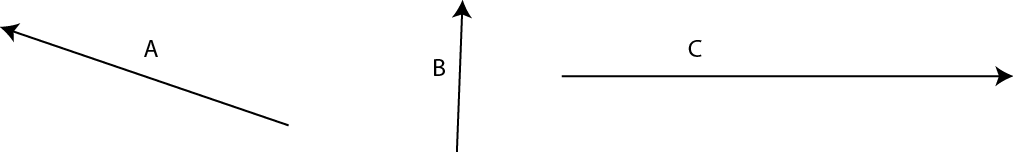
\includegraphics[width=6cm]{figs/ThreeVectors}
\end{marginfigure}

\be
\item $\vec{A} + \vec{B}$

\item $\vec{A}-\vec{C}$

\item $\vec{A} \cdot \vec{B}$

\item $(\vec{A} \times \vec{B}) \times \vec{C}$

\item $(\vec{A} \cdot \vec{B}) \times \vec{C}$

\ee

\item {\bf Cartesian Vectors:}  Let $\vec{A} = 3 \hat{\imath} + 4 \hat{\jmath}$, $\vec{B} = \hat{\imath} -\hat{\jmath}$, and $\vec{C} = -5 \hat{\jmath}$. Find the results of identified operations, or (if appropriate) identify the operation as nonsense.

\be
\item $ | \vec{A} + \vec{B}| $

\item $\vec{A} \times \vec{C}$

\item $\vec{A} \cdot \vec{B}$

\item $(\vec{A} \times \vec{B}) \times \vec{C}$

\item $(\vec{A} \times \vec{B}) \cdot \vec{C}$

\ee

\item {\bf Vector Construction:} $\vec{A}$ and $\vec{B}$ are two arbitrary, non-parallel vectors in three-dimensional space. Using them, construct the following vectors (i.e., find mathematical expressions for the specified vector in terms of the vectors $\vec{A}$ and $\vec{B}$ ) :

\be
\item The vector $\hat{A}$, which has a length of 1, and points in the direction of $\vec{A}$.

\item The vector $\hat{n}$, which has a length of 1, and is perpendicular to both $\vec{A}$ and $\vec{B}$.
\ee

%\item {\bf Using vectors to describe positions:}  Make a sketch of the system consisting of the inner solar system.  Set the origin on the sun and assume the sun is stationary.  Include Mercury, Venus, Earth, and the Earth's moon (no need to be to scale here), and assume that everything is in the $xy$ plane, and that all orbits are circular.
%
%\be
%\item Sketch the following position vectors: 
%\bi
%\item The displacement vectors of all three planets from the sun (call these $\vec{M}$, $\vec{V}$, and $\vec{E}$)
%\item The displacement vector of the moon from the earth (label this $\vec{m}$).
%\ei
%\item With these definitions in place, sketch and find expressions (just in terms of $\vec{M}$, $\vec{V}$, and so forth) for:
%\bi
%\item The displacement vector pointing from the Earth to Venus
%\item The displacement vector from Venus to the moon
%\ei
%\item Find (i.e., make up) a mathematical expression for the following vector quantities as a function of time $t$ where $t$ is given in days  (in other words, come up with a {\it vector-valued function of time}, like $\vec{r}(t) = t^2 \,\hat{i} + \log t \,\hat {j}$, which has the right properties to describe an orbit).
%\bi
%\item The displacement vector of the Earth with respect to the Sun, assuming that at $t=0$ the displacement is given by $d_E \hat{i}$
%\item The displacement vector of the moon with respect to the Sun, assuming that at $t=0$ the displacement is given by $(d_E + d_M) \hat{i}$
%\item The velocity vector of the Earth with respect to the Sun.
%\item The velocity vector of the moon with respect to the Sun.
%\ei

\ee


%\item{\bf Vectors to Describe Directions:} A final project in ModSim involved trying to model the motion of a rollercoaster cart, with a suspension, on a track.  If you think about it, the forces in this situation act in a variety of different directions:  the suspension acts perpendicular to the track; fricitional forces will act parallel to the track, etc.
%
%As a consequence, it is necessary to decide, for any given location of the cart, what the ``normal'' direction is, and what the parallel direction is.
%
%The diagram shows one way to abstract this:  The track is described by a function $f(x)$.  The cart is abstracted to a point mass, located at some location above the track, and attached to the track by a spring and a damper that are perpendicular to the track. 
%
%\begin{marginfigure} \includegraphics[width=6cm]{figs/rollercoaster}
%\end{marginfigure}
%\be
%
%\item First, let's consider the simple case that we know the position of the cart on the track -- i.e., the cart's contact point is $(x, f(x))$.  For this case, find an expression for the unit vector $\hat{t}$, which is parallel to the track's surface, and the unit vector $\hat{n}$, which is perpendicular to the track's surface.  Hint:  it might help you to think about the position vector of the cart, the velocity vector of the cart, and the direction of the velocity of the cart.
%
%\item Now assume that you need to find the contact point.  In other words, you know where the center of mass of the cart is located (some position $\vec{r} = x \hat{\imath} + y \hat{\jmath}$ which is above the  track), but you don't know what the contact point is. You do, however, know that the vector connecting the contact point and the center of mass is perpendicular to the track.  Propose a set of steps that you could follow to determine the 
%the contact point, and accordingly, $\hat{t}$ and $\hat{n}$.  Is the contact point uniquely defined?
%
%\item This question actually gets at a pretty important general idea, which is finding a vector that points along a curve.  Let's do one other example.  Consider the case of a curve described by 
%$$\vec{r}(t) = t \cos t \hat(i) + t \sin t \hat{j} $$
%Find an expression for the unit vector that is tangent to the curve $\vec{r}$ for any given time $t$.
%
%\item If you're feeling particularly MATLAB-ish, write a piece of code that, given $x$, $y$, and $f(x)$, will determine the contact point, and produce plots that show that it works.  This is an optional question.
%
%
%\ee
 

\section{Forces: Ideas and Models}


Whether we're discussing a static situation in which stuff doesn't move, or a dynamic situation in which stuff does move, we still need to think about the ways in which the stuff we are concerned with (the {\it system} interacts with the rest of the universe.  There are a set of videos on the website that deal with the idea of forces and models for forces.  Watch these videos, and then do an appropriate number of  the exercises below.



\begin{enumerate}[resume]
\item Consider a sprinter who is running (and accelerating) over a level surface.  What fundamental forces are acting on the sprinter (or parts of the sprinter)?  How do these translate into phenomenological forces?  How large might these different forces be?  What force is responsible for accelerating the runner forward?

\item ``I am pushing a coffee cup across my desk.  Since it is in motion, I know that the magnitude of the frictional force acting on the cup is given by $\mu_k N$, where $\mu_k$ is the coefficient of kinetic friction and $N$ is the normal force the table exerts on the cup.''  True or false?  Discuss, and use a free body diagram to explain.

\item ``I am pushing on a coffee cup that is sitting on my desk.  Since it is not moving, I know that the magnitude of the frictional force acting on the cup is given by $\mu_s N$, where $\mu_s$ is the coefficient of static friction and $N$ is the normal force the table exerts on the cup.''  True or false?  Discuss, and use a free body diagram to explain.

\item Your physicist friend tells you, ``Newton's third law says that for every force there is an equal and opposite force.  For example, when an object is sitting on the ground, the force exerted by gravity ($-mg \hat{j}$), is exactly offset by the normal force ($+mg \hat{j}$).''  How do you respond to your friend's claim?  Is she right?  Wrong?  Why?

%\item On earth, we use the gravitational force model $F=-mg$, where $g= 9.8$ m/sec$^2$.  What would $g$ be if earth were made out of the same kind of material, but had twice the radius? 
%
%
%\item Typically springs are modeled with $F = - k(l-l_0) \hat{s}$.  Find an actual physical spring (i.e. something that you might normally choose to model as a spring), and test it using one of the force sensors that we have in the studio.  Where does the spring model break down for the object you chose?  Propose a better functional model for the spring you chose.

\begin{marginfigure}
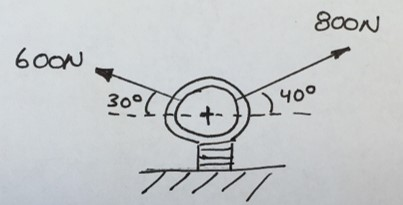
\includegraphics[width=6cm]{figs/inter1_eyescrew.jpg}
\end{marginfigure}
\item Two forces are applied to an eye hook. They lie in the plane of the page with the orientation and magnitudes as shown. Determine the orientation and magnitude of the net or resultant force acting on the hook. 
%Use two approaches:
%\be
%\item The geometry of triangles (e.g., law of sines and cosines)
%\item The components in a Cartesian coordinate system.  
%\ee


\item A man is pulling a rope running between points A and B with a force of 70 lbs. Describe this force as a vector in terms of components aligned with the x-y-z coordinate system shown. 
\begin{marginfigure}
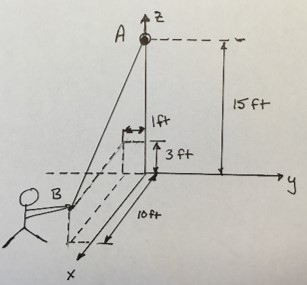
\includegraphics[width=6cm]{figs/inter1_cablepull.jpg}
\end{marginfigure}

%\item In the videos we discussed a couple of kinds of constraint forces: the ``normal force'', and the ``static frictional force''.  Consider a piece of paper that is pinned to the wall with a single push pin: you can rotate it, but you can't take it off the wall without ripping it or removing the pin. What are the constraint forces acting on the paper?  What directions do they take?


\end{enumerate}


\section{Moments: Ideas and Calculating}

Moments (which you may previously have heard referred to as ``torques'' -- same thing -- are sort of the rotational analog to forces: just as forces cause linear acceleration, moments cause angular acceleration.  You can think about moments both as a result of applying forces (when you apply a force to an object, you are also applying a moment to the object); you can also think about externally applied moments that do not have associated net external forces (e.g., when a motor applies a torque to a wheel).

There are a set of videos about the ideas around moments and how to calculate them (yay, cross products).  Watch these, and then do an appropriate number of  the problems below.

\begin{enumerate}[resume]
\begin{marginfigure}
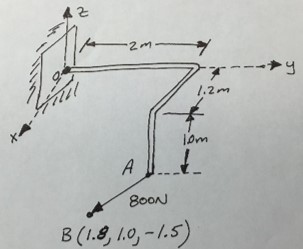
\includegraphics[width=6cm]{figs/Inter1_mom-beam.jpg}
\end{marginfigure}
\item A multi-section beam is attached to a wall. What is the moment about point $O$ created by the 800 N force action on point $A$ as shown? 
 



\begin{marginfigure}
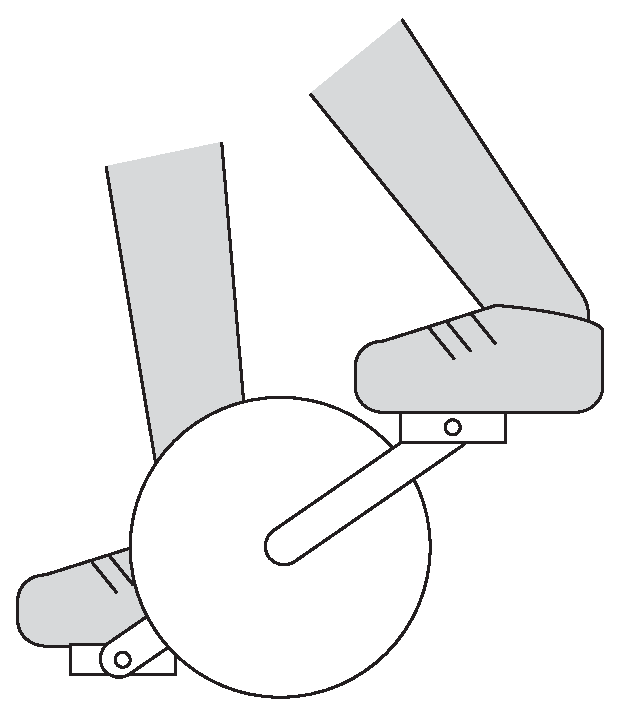
\includegraphics[height=1in]{figs/BikePedal1}
\end{marginfigure}
\item Imagine that you are riding a bicycle (without cleats or toe clips).  At what point during a pedaling cycle is the moment on the crank generated by your feet on the pedals greatest (assume you are calculating the moment about the center point of the crank)?  When is it least?  What is the direction of the moment?  Think about this both in 2D and in 3D: how do your answers differ, and why?

\item (Think in 2D for this one): As you step on the pedal, the moment you apply to the crank is offset a moment produced by tension in the chain -- thus, the tension in the chain is proportional to the moment you apply to the crank.  This tension, in turn, applies a moment to a cog attached to the rear wheel.  Which cog, $A$ or $B$, will yield the highest moment on the rear wheel?  What will the direction of this moment? 
\begin{marginfigure}
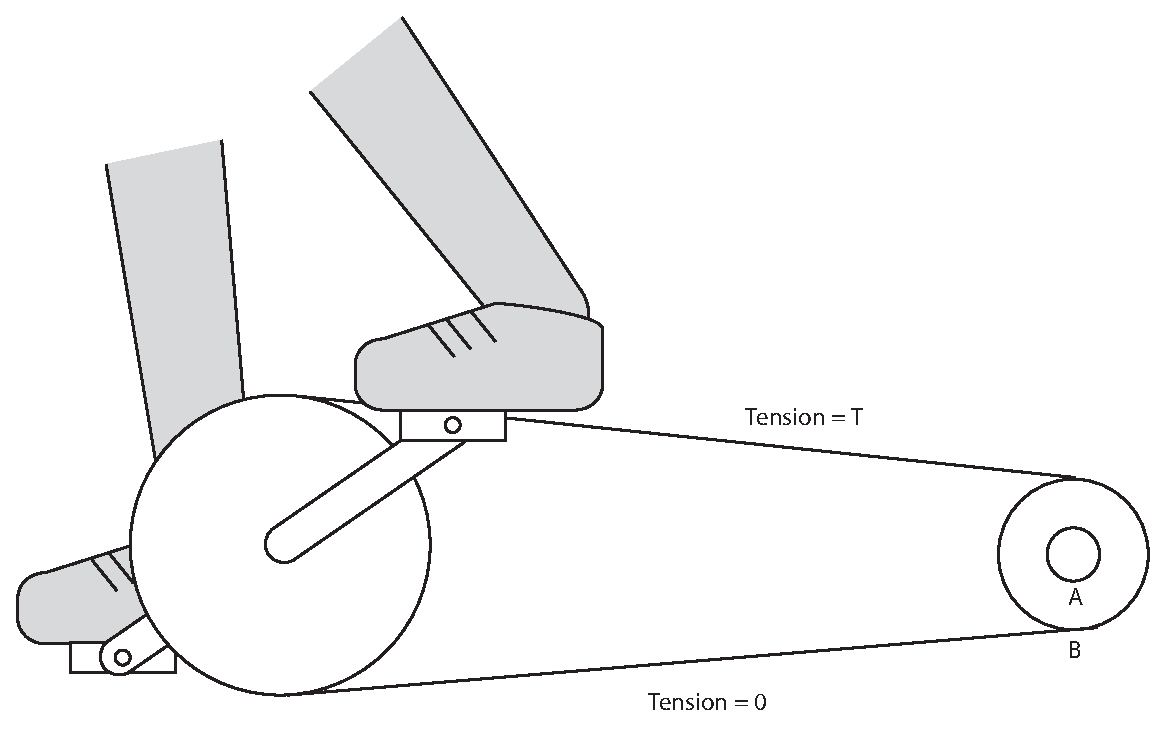
\includegraphics[width=6cm]{figs/BikePedal2}
\end{marginfigure}

\item Why are multi-speed bikes desirable?  Given the answer to above, it seems like a pretty simple design would yield very high moment on the rear wheel.  Isn't this always desirable, since this means you can exert more force against the ground, and hence accelerate faster?

%\begin{marginfigure}
%\includegraphics[width=6cm]{figs/inter1_bike-photo.jpg}
%\end{marginfigure}
%\item Why would one downshift (switch to a larger diameter gear in the rear) going up a steep hill? 
%

 

\item What might a 1000 N-m torque wrench look like?   Why?  Propose a nominal design (size, configuration, etc.).

%\begin{marginfigure}
%\includegraphics[width=6cm]{figs/inter1_boat-photo.jpg}
%\end{marginfigure}
%\item Sailboats often have keels and rudders. The rudder is used to steer the boat. What is purpose of the keel? What is the relationship between the depth of the keel, the size of the sails, and the speed of the boat? 
%
 


%\item On a sailboat, the equivalent force of the wind on the sail can be thought of as a lift force $\vec{L}$ and a drag force $\vec{D}$ that both operate at the center of pressure of the sail.  The drag force is in the direction $\hat{v}_A$, where $\vec{v}_A$ is the apparent wind velocity, and the lift force is perpendicular to $\hat{v}_A$.  Sketch a sailboat that is close-hauled, and sketch the directions of the apparent wind and the directions of the forces acting on the sails.  Then sketch the directions of the moments generated by these forces about the sailboat's center of mass.  You may want to make sketches from different perspectives in order to get your head wrapped around this.
%
\end{enumerate}

%%%%%%%%%%%%%%%%%%%%%%
% SECTION 3: DRAWING FREE BODY DIAGRAMS
%%%%%%%%%%%%%%%%%%%%%%

\clearpage

\section{Free Body Diagrams}

A key piece of abstracting mechanical systems is the ability to choose and draw an appropriate free body diagram for your system.  As with most modeling work, you need to make choices in representing the system: what forces will you include, and what forces will you ignore?  Will you think about distributed forces or equivalent forces?

There are a set of videos on creating FBDs.  Watch these and then proceed to do an appropriate number of  the problems below.

\begin{enumerate}[resume]
%\item Consider a sprinter who is running (and accelerating) over a level surface.  In the space below, draw a free body diagram for the person (assume one of the person's feet is in contact with the ground).  Use appropriately directed arrows, in appropriate places, and of appropriate sizes to indicate the forces acting on the person, and label the arrows appropriately.  

%\item Consider a hot air balloon carrying a basket with two riders.  It is floating at a given altitude.  Draw free body diagrams for the following:
%\be
%\item Draw a FBD for the whole system (balloon + basket) using equivalent forces to represent all distributed (body and contact) forces.
%\item Draw an FBD for the basket using equivalent forces to represent all distributed forces.
%\item Draw a FBD for the balloon (not including the basket) using distributed forces.
%\item Comment on the utility of each of these FBDs: what questions would each help you to answer?
%\ee


\item Recall the multi-section beam in the previous section (question 15).  Draw a free body diagram of multi-section beam in the previous section. Under what conditions would it be reasonable to neglect the weight of the beam?   Why?

\begin{marginfigure}
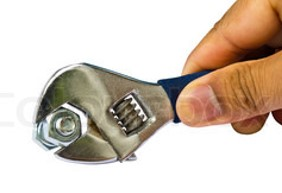
\includegraphics[width=6cm]{figs/inter1_wrench.jpg}
\end{marginfigure}

\item The picture at the right shows a person trying to remove a nut with a wrench.  Draw a free body diagram for 
\be \item The wrench only
\item The nut only 
\ee
Then, using your FBD?s, explain how the wrench is used to remove the nut. 
 

\item Consider a bike that is stationary with a rider standing on the pedals (see below). Draw a complete FBD for the crankset.  Sketch your vectors such that your FBD appears to satisfy the equilibrium condition.

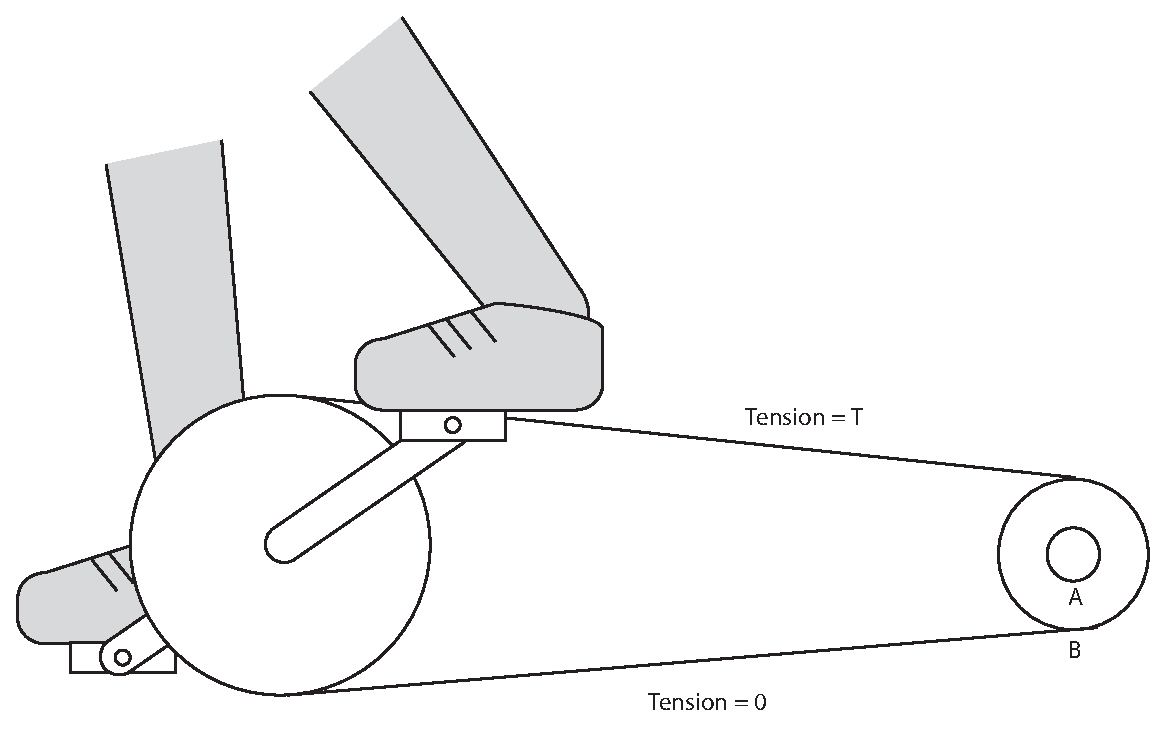
\includegraphics[height=1.5in]{figs/BikePedal2}

\item The diagram at right shows a front-wheel drive car on a hill.  The car is in drive, but is not moving: the brakes are engaged.

\begin{marginfigure}

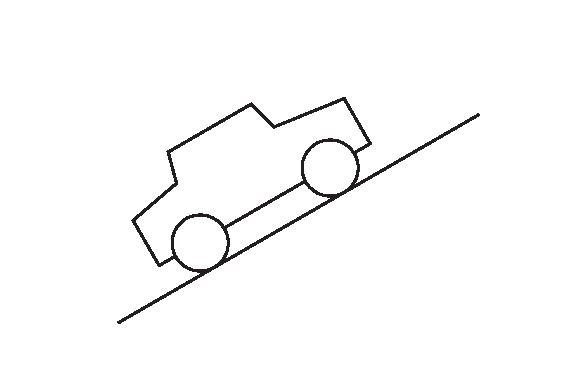
\includegraphics[width=2in]{figs/CarOnHills}

\end{marginfigure}

Draw free-body diagrams for the following systems:

\begin{enumerate}
\item System = the entire car.

\item System = a rear wheel, hub, and rotor of the car. Assume a disc brake, as shown at right.  Note that when the brake is engaged, the caliper pinches the rotor between the brake pads.

\item System = a front wheel, hub, and rotor of the car. Assume a disc brake, as shown at right.  Note that when the brake is engaged, the caliper pinches the rotor between the brake pads.  Remember that it's a front-wheel drive car in drive!
\begin{marginfigure}
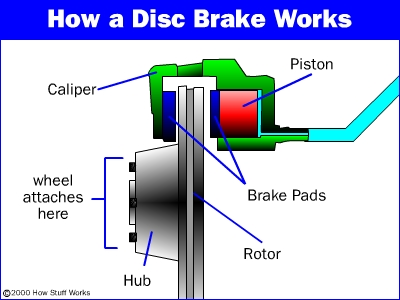
\includegraphics[width=2in]{figs/disc-brake3.jpg}

\caption{Cross section of disc brake, from {\tt howstuffworks.com}} 
\end{marginfigure}
\end{enumerate}

%
%\item A chain, consisting of $N$ links, each of mass $m$, hangs from the ceiling.  Draw an FBD for the following system definitions:
%\be
%\item The entire chain
%\item The $n$th link in the chain ($n=1$ for the chain that is attached to the ceiling; $n=N$ for the lowest link in the chain), for $n=1$, $n=N$, and $n=i$ where $1 < i < N$
%\ee

\item A pin joint or pin connector is a mathematical idealization of the interaction between two connected bodies. The two bodies can rotate freely relative to one another about an axis passing through the pin joint. It does not allow relative motion between the bodies. Wheels rotating on axels or bearing are often modeled as pin joints. See the .pdf document on the website which describes pin joints and various other supports. 

Find a real connection or support that can be modeled as a pin joint and take a photo of it. Draw a free body diagram of the pin between the two bodies. What idealizations must be made so that this representation can be made? 

\begin{marginfigure}
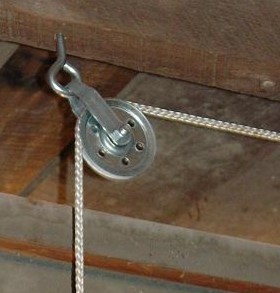
\includegraphics[width=2in]{figs/inter1_pulley.jpg}
\end{marginfigure}

\item The diagram at the right shows a rope routed over a pulley wheel that is suspended from a bracket by a pin connector. Draw a free body diagram the wheel of the pulley.
 


%\item You've decided to model a zipline. 
%
%
%\be
%\item As a first pass, use the abstraction at the right: The rider is a rigid body, hanging off of the cable; the cable does not deform.  
%
%\begin{marginfigure} 
%\includegraphics[width=6cm]{figs/zipline}
%\end{marginfigure}
%Create a free body diagram for the zipline rider in this abstraction.  Explain all of the forces and moments in your diagram.
%
%\item Now take a second pass at modeling the rider.  What might be a more realistic free body diagram, and why?
\ee



\clearpage

\end{document}

\section{Statics}

Now that you've dealt with forces and moments, and you've done some drawing of free-body diagrams, let's apply these ideas to static conditions.

\begin{enumerate}[resume]


\begin{marginfigure} 
\includegraphics[width=6cm]{figs/Inter1_boxhang.jpg}
\end{marginfigure}

\item A box weighing 200 lbs is being supported by two cables, ab and cb. The angles of the cables with respect to the horizontal are shown. What is the tension in the cables such that the sum of all three force vectors equals zero? What does this say about the motion of the mass?  Assume that the length of the cables is constant and the suspension points a and c are moved to the left and right, respectively. Do you expect the tension in the cables to increase, decrease, or stay the same? Do a calculation to verify your answer. 

\item What are three types of sensors can that be used to measure force? Identify a specific sensor that you could purchase that could be used to measure the tension predicted in cable ab in the previous question. Download a copy of that sensor?s data sheet or specifications and put a copy in your portfolio. 


\item Consider the system shown below.  It consists of a mass $m_1$ on a table, attached via a string to a mass $m_2$ beneath the table.  The system is initially at rest.  Assume that you can use a standard frictional model with a coefficient of static friction $\mu_s$ and a coefficient of kinetic friction $\mu_k$.

\begin{marginfigure} 
\includegraphics[width=6cm]{figs/BallOnTable}
\end{marginfigure}

By drawing free body diagrams and applying statics conditions, determine the conditions (i.e., values of parameters $m_1$, $m_2$, $\mu_s$, and $\mu_k$) for which the system remains at rest.

\item Consider the situation shown at the right.  What is the minimum torque required for the motor to be able to move the weight (either by tipping it or dragging it)?  If you wanted to minimize the required torque, at what height would you put the 10 cm pulley?


\begin{marginfigure} 
\includegraphics[width=6cm]{figs/MotorWeightStatics}
\end{marginfigure}

\item Consider a block on a ramp, as shown below.  The ramp is free to move.  There is a frictional interaction between both the the block and the ramp and between the ramp and the ground.  \begin{marginfigure} 
\includegraphics[width=3in]{figs/BlockOnRampSimple}
\end{marginfigure}

\be
\item Consider the case that both the block and the ramp are stationary.  Find the necessary coefficients of friction to maintain this static condition.

\item Where is the equivalent contact force from the ground on the ramp applied?  How large and in what direction is this force?

\item Now consider the case that the block has started to slide down the ramp.  What are the necessary conditions for the ramp to remain stationary?  Where is the equivalent contact force from the ground on the ramp applied?  How large and in what direction is this force?

\ee

\ee
\section{Thinking about distributed forces}

We often determine the equivalent force for distributed forces (body and contact forces) by thinking about how big the total force is, and where the force is applied.  For example, gravity is a distributed force that acts at the center of mass; buoyancy is a distributed force that acts at the center of buoyancy; drag acts a the center of pressure, etc.  

 

\end{document}